\documentclass[onecolumn]{article}

%Titling
    \usepackage[compact]{titlesec}
    \titlespacing{\section}{0pt}{3ex}{2ex}
    \titlespacing{\subsection}{0pt}{2ex}{1ex}
    \titlespacing{\subsubsection}{0pt}{1ex}{0.5ex}
\titleformat*{\section}{\Large\scshape}
\titleformat*{\subsection}{\Large}
\titleformat{\subsubsection}[runin]
  {\normalfont\bfseries}{\thesubsection}{1em}{}
  
%Page size
	\addtolength{\oddsidemargin}{-.875in}
	\addtolength{\evensidemargin}{-.875in}
	\addtolength{\textwidth}{1.75in}

	\addtolength{\topmargin}{-.875in}
	\addtolength{\textheight}{1.75in}
	
	\parskip=.1cm
	
%Indented paragraph
\setlength{\parindent}{0pt}
\newenvironment{indentpar}[1]
  {\begin{list}{}
          {\setlength{\rightmargin}{#1}}
          \item[]
  }
  {\end{list}}

\usepackage{graphicx}
\graphicspath{ {figures/} }
\usepackage[T1]{fontenc}
\usepackage{lmodern}
\usepackage{float}
\usepackage[table]{xcolor}
\usepackage{multirow}
\usepackage{tabularx} 
\usepackage[table]{xcolor}
\usepackage[font=small,labelfont=bf]{caption}
\usepackage{textcomp}
\usepackage{gensymb}
\usepackage{lineno}
\usepackage{amsmath}
\usepackage{blindtext}
\usepackage{texshade}
\usepackage{bigdelim}
\usepackage{textgreek}
\usepackage{multicol}

% tikz setup
\usepackage{tikz}
\usetikzlibrary{shapes,arrows}
\newcommand*{\h}{\hspace{5pt}}% for indentation
\newcommand*{\hh}{\h\h}% double indentation


%Citations
\usepackage[authoryear]{natbib}
\setcitestyle{authoryear,open={(},close={)}}
\renewcommand{\bibname}{References}

\usepackage[allbordercolors = white, linkcolor = blue, citecolor = blue, colorlinks = true]{hyperref}
\usepackage[nameinlink]{cleveref}

%titling
\title{Modelling Uncertainty in the Risk of Intensive Care Unit Readmission I: Data Extraction and Modelling}
\date{\today}
\author{Ben Cooper}


\begin{document}
\maketitle

\section{Introduction}

% Brief background on ICU risk stuff
Unplanned readmission to an intensive care unit (ICU) during the same hospital admission is a relatively common event, affecting between 1.3\% and 13.7\% of all ICU patients \citep{Elliott2014}. Not only do readmissions to ICU represent a substantial strain on hospital resources, but also readmitted patients tend to have worse prognoses, increased length of ICU stay, and greater risks of morbidity and mortality \citep{MarkaziMoghaddam2020}. Despite this, the precise factors contributing to ICU readmission risk remain unclear. Several models for risk prediction have been developed which tend to use very different variable sets, and no model has been widely externally validated. Accordingly, this project does not aim to develop or validate a novel model for ICU readmission, but to tackle an issue that affects the implementation and interpretation of all risk prediction models - how to deal with missing or incomplete data in the predictor variables \citep{Steyerberg2008}.

\subsection{Scope and Aims of Phase I}

This document provides a written overview of the first phase of the project. The aims of this phase were twofold:

\begin{enumerate}
\item To extract a dataset from the MIMIC-III database of surgical ICU patients, consisting of a clearly defined outcome measure (ICU readmission), and a range of predictors.
\item To compare the performance of a range of published models for the prediction of ICU readmission risk and identify the best model to take forward. This will form the prediction model at the core of a system for quantifying uncertainty and dealing with missing data.
\end{enumerate}


\subsection{Readmission prediction models}

% Overview of structure, strengths and shortcomings of each model
This report will investigate five models for ICU risk prediction. I will give a brief overview of all five here. Further details on their predictors, statistical approaches and validations are given in \Cref{CandidateModels}. Henceforth, all models will be referred to by the name of the first author, with the exception of the APACHE-II system.
% APACHE-II
The first `model' is the APACHE-II scoring system devised by \cite{Knaus1985}. `Model' is used in inverted commas, as this model was not designed for predicting ICU readmission risk, but instead is a general system to score the severity of a patient's condition using 12 routine physiological variables, age, and medical history. Increasing APACHE-II score has been shown to correlate well with increasing risk of in-hospital mortality for ICU patients. 
% Frost
\cite{Frost2010} used a logistic regression model to develop a nomogram for predicting ICU readmission risk based on 14,952 patients in a single hospital in Australia. Unfortunately, as they do not present the coefficients from their model directly, only in the form of the nomogram, several of these coefficients can only be approximated, which may hinder external validation of the model.

% Fialho
\cite{Fialho2012} developed a model using data mining and fuzzy logic approaches with the MIMIC-II database, precursor to the MIMIC-III used here. Their model focusses on the values of physiological variables during the 24 h before discharge. The fuzzy rules provide a significant barrier to external validation, however.
% Martin
\cite{Martin2018} also developed their model into a nomogram, but unlike Frost, also provided coefficients and a precise formula to generate risk estimates. Their model used 3,109 patients in a single academic centre, and narrowed an initial 179 candidate variables down to 7 variables, covering demographics, physiological measurements and medical history.
% Hammer focussed on modifiable variables
Finally, \cite{Hammer2020} developed the `RISC' score (Readmission to the
Intensive care unit in Surgical Critical care patients, henceforth simply called `Hammer' for consistency with other models) using logistic regression. Their model aimed to include a number of modifiable variables to aid its use as a clinical tool.

\section{Methods}

\subsection{Data Source}

% Overview of MIMIC data
This work uses the open-access MIMIC-III critical care database \citep{Johnson2016}, which comprises ICU stay information for 61,532 adult patients at the Beth Israel Deaconess Medical Centre between June 2001 and October 2012. The database includes information such as demographics, vital sign measurements made at the bedside ($\sim$1 data point per hour), laboratory test results, procedures, medications, caregiver notes, imaging reports, and mortality (both in and out of hospital).

\subsection{Inclusion criteria}

% Workflow in extract_patients & preprocess_data
An overview of inclusion and exclusion criteria is shown in \Cref{Flowchart}. In brief, we initially include all patients admitted under or transferred to a surgical service, and who underwent a surgical procedure either during or prior to an ICU stay. We exclude patients with invalid surgical procedure codes, or procedure types with <20 patients in the dataset. We also exclude patients whose surgical procedure took place after their last ICU stay, or who died during the same hospital admission as their ICU stay. Finally, we exclude patients with data in any of the following categories:

\begin{itemize}
\item Missing entire hospital record
\item Missing assessment data for predictors
\item Missing measurement data for predictors within 24 h prior to ICU discharge
\item Physiologically impossible or implausible measurements
\end{itemize}

% Flowchart------------
\begin{figure}
\centering
  \caption{Flowchart of inclusion and exclusion criteria for patients in the dataset, alongside sample sizes at each step.}
  % setting the typeface to sans serif and the font size to small
  % the scope local to the environment
  \sffamily
  \footnotesize
  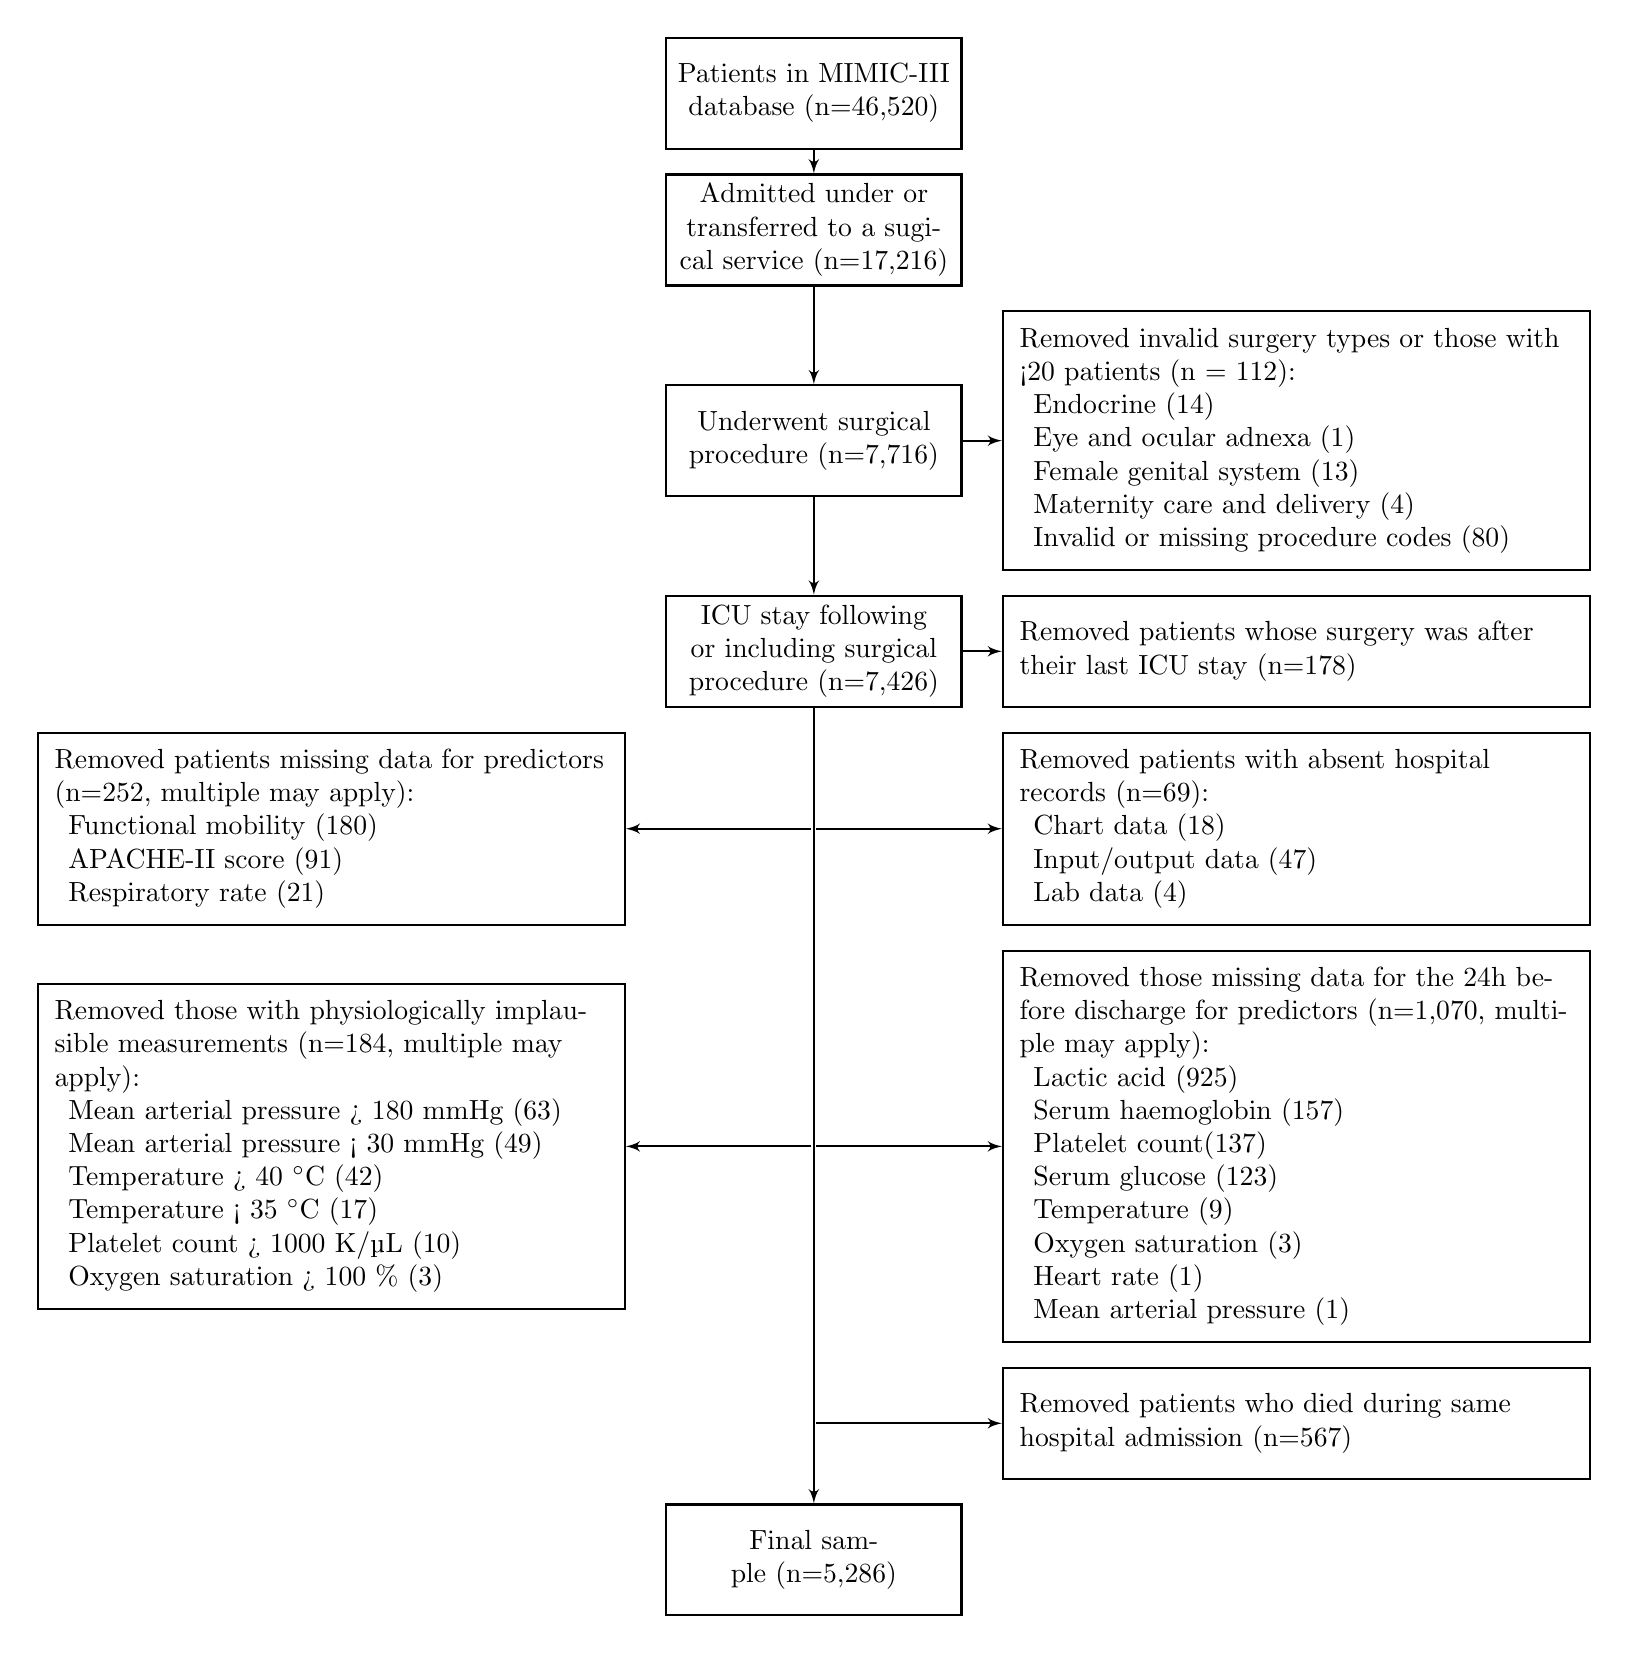
\begin{tikzpicture}[auto,
    block_center/.style ={rectangle, draw=black, thick, fill=white,
      text width=10em, text centered,
      minimum height=4em},
    block_left/.style ={rectangle, draw=black, thick, fill=white,
      text width=20em, text ragged, minimum height=4em, inner sep=6pt},
      line/.style ={draw, thick, -latex', shorten >=0pt},
          block_noborder/.style ={rectangle, draw=none, thick, fill=none,
      text width=-4em, text centered, minimum height=1em}]
    % outlining the flowchart using the PGF/TikZ matrix funtion
    \matrix [column sep=5mm,row sep=3mm] {
      % row 1
      & \node [block_center] (full) {Patients in MIMIC-III database (n=46,520)};\\
      % row 2
      &\node [block_center] (service) {Admitted under or transferred to a sugical service (n=17,216)}; \\
      % row 3
      &\node [block_center] (procedure) {Underwent surgical procedure (n=7,716)};       
      & \node [block_left] (invalidprocedure) {Removed invalid surgery types or those with <20 patients (n = 112): \\
        \h Endocrine (14)\\
        \h Eye and ocular adnexa (1)\\
        \h Female genital system (13)\\
        \h Maternity care and delivery (4)\\
        \h Invalid or missing procedure codes (80)
        }; \\
      % row 4
        &\node [block_center] (icuprocedure) {ICU stay following or including surgical procedure (n=7,426)};       
      & \node [block_left] (procedure_after_icu) {Removed patients whose surgery was after their last ICU stay (n=178)}; \\
      % row 5  
        \node [block_left] (missing_predictors) {Removed patients missing data for predictors (n=252, multiple may apply):\\
		\h Functional mobility (180)\\
		\h APACHE-II score (91)\\
		 \h Respiratory rate (21)}; &
       \node [block_noborder] (hidden_r5) {};&
      \node [block_left] (absent_charts) {Removed patients with absent hospital records (n=69): \\
        \h Chart data (18)\\
        \h Input/output data (47)\\
        \h Lab data (4)
        }; \\  
        % row 6 
        \node [block_left] (implausible) {Removed those with physiologically implausible measurements (n=184, multiple may apply): \\
		\h Mean arterial pressure > 180 mmHg (63)\\
	 	\h Mean arterial pressure < 30 mmHg (49)\\
		\h Temperature > 40 $^\circ$C (42)\\
		\h Temperature < 35 $^\circ$C (17)\\
		\h Platelet count > 1000 K/$\micro$L (10)\\
		\h Oxygen saturation > 100 \% (3)
        };   &
           \node [block_noborder] (hidden_r6) {};&
      \node [block_left] (missing_24h) {Removed those missing data for the 24h before discharge for predictors (n=1,070, multiple may apply): \\
		\h Lactic acid (925)\\
		\h Serum haemoglobin (157)\\
		\h Platelet count(137)\\
		\h Serum glucose (123)\\
		\h Temperature (9)\\
		\h Oxygen saturation (3)\\
		\h Heart rate (1)\\
		\h Mean arterial pressure (1)
        }; \\  
        % row 7  
       &
       \node [block_noborder] (hidden_r7) {};&
       \node [block_left] (mortality) {Removed patients who died during same \mbox{hospital} admission (n=567)}; \\
        % row 8  
       &
       \node [block_center] (final) {Final sample (n=5,286)};& \\  
      };
    % end matrix
    % connecting nodes with paths
     \begin{scope}[every path/.style=line]
      \path (full)   -- (service);
      \path (service) -- (procedure);
      \path (procedure) -- (icuprocedure);
      \path (procedure) -- (invalidprocedure);
      \path (icuprocedure) -- (procedure_after_icu);
      \path (hidden_r5) -- (absent_charts);
      \path (hidden_r5) -- (missing_predictors);
      \path (icuprocedure) -- (final);
      \path (hidden_r6) -- (implausible);
      \path (hidden_r6) -- (missing_24h);
      \path (hidden_r7) -- (mortality);
    \end{scope}  
  \end{tikzpicture}
  \label{Flowchart}
\end{figure}

\subsection{Outcome measure}

% Workflow in define_outcomes
The `readmission' outcome measure is defined as patients readmitted to the ICU within the same hospitalisation event. Thus, patients discharged fully from the hospital and then readmitted are excluded, even if they were then readmitted to ICU. This is the same outcome measure used by the Frost and Hammer models, whilst the Martin and Fialho models use any readmission within 72 h of discharge.
% All models but martin use within same hosp (martin == 72h)

\subsection{Candidate models}
\label{CandidateModels}

Here, I will give an overview of each model, as well as the model performance metrics given in the paper deriving each model (with the exception of APACHE-II). In general, the performance of binary prediction models can be measured in two separate but related metrics using an unseen validation dataset. Discrimination is usually measured as the area under the Receiver Operating Characteristic curve (called AUROC or AUC). It measures the model's ability, when presented with two patients, one of whom was readmitted and one of whom was not, to give a greater probability of readmission to the patient who was readmitted. Its values range from 0.5, indicating a model no better than guessing, to 1, indicating perfect discrimination. Crudely, discrimination can be classified as poor (0.5--0.6), moderate (0.6--0.7), good (0.7--0.8), very good (0.8--0.9) and excellent (>0.9).

Calibration measures the agreement between a model's predicted readmission, and observed readmission. This is usually performed by splitting patients into deciles based on assigned readmission probability, then comparing observed to expected readmission rates within each decile. This goodness-of-fit can then be formally assessed using a Hosmer-Lemeshow Chi-squared ($ \chi^{2} $) test, with a well-calibrated model showing no significant differences between observed and expected readmission.

For each model I also present a cross-tabulation of the model's predictors with readmission status from the MIMIC-III dataset, to demonstrate the expected relationship between each predictor and readmission.

% Overview of APACHE-II system
\subsubsection*{APACHE-II.}

The APACHE-II system was not designed to specifically predict ICU readmission, but rather to assess the severity of a patient's condition. Nonetheless, it has shown to be an informative predictor of ICU readmission \citep{Campbell2008}, and as such is used in both the Hammer and Frost models. This makes it a good `baseline' predictive model to compare others too. It comprises a scoring system across 12 variables: Core temperature, mean arterial pressure, heart rate, respiratory rate, oxygenation (arterial partial pressure if fraction of inspired oxygen < 0.5, else arterial-alveolar gradient), arterial pH, serum sodium, serum potassium, serum creatinine, haematocrit, white blood cell count and Glasgow coma score. Serum bicarbonate levels are also used if arterial blood gas measurements are not present.

Each variable scores 0 if in a `normal' range, with increasingly higher scores for abnormally low or high values. The worst value for each variable in the preceding 24 h is used to determine the score. Additional points are then given for increasing age, emergency admissions and the presence of certain comorbidities. The resulting score falls between 0 and 71, with higher values indicating a more severe condition.


% Outline each model and its predictors and AUC/calibration
\subsubsection*{Frost.} 

The Frost model is based on a logistic regression model, and includes the following variables (\Cref{Table1Frost}): Age, sex, elective admission (yes/no), admission source (Operating theatre/recovery ward, emergency department, other hospital or general ward), APACHE-II score at discharge, ICU stay duration > 7 days (yes/no), discharge outside the hours of 08:00--16:00, and acute renal failure during ICU stay (yes/no). Each variable carries a number of points, the sum of which is used to determine readmission risk. Unfortunately, the coefficients linking variables to score, and total score to readmission risk are not presented, and must be inferred from the nomogram. In most cases, variables map clearly onto discrete score values. However, the mapping between total score and readmission is neither linear, nor fully exponential. This relationship has been approximated in my workflow, but may result in poor calibration. The authors report moderate discrimination (AUC = 0.66), and do not quantitatively report calibration, only describing it as `good'.

\begin{table*}[h]
\centering
	\renewcommand{\arraystretch}{1.4}
		\caption{Cross-tabulation of variables in the Frost model with ICU readmission status in the MIMIC-III dataset. Continuous variables are presented as means $\pm$ standard deviation. The APACHE-II is measured at or close to discharge.}
	\begin{tabular}{lp{2.5cm}p{2cm}}
		\hline
		Variable & No Readmission & Readmitted to ICU\\
		\hline
		N & 4944 (93.5\%)  &      342 (6.5\%)\\
		Age & 64.2 $\pm$ 14.5 & 63.5 $\pm$ 14.5\\
		Sex &&\\
		\quad Male & 3121 (63.1\%)   &    207 (60.5\%)\\
		\quad Female & 1823 (36.9\%)  &     135 (39.5\%)\\
		Elective admission & 1980 (40\%)  &     104 (30.4\%)\\
		Admission source &&\\
		\quad Operating theatre &2246 (45.4\%)    &   120 (35.1\%)\\
		\quad Emergency room &769 (15.6\%)  &      91 (26.6\%)\\
		\quad Other hospital &976 (19.7\%)    &    69 (20.2\%)\\
		\quad Ward &953 (19.3\%)   &     62 (18.1\%)\\
		APACHE-II score & 10.4 $ \pm $ 4.70 & 12.0 $ \pm $ 4.87\\
		ICU stay >7 days & 864 (17.5\%)   &     98 (28.7\%)\\
		Discharged after hours & 2874 (58.1\%)    &   223 (65.2\%)\\
		Acute renal failure & 788 (15.9\%)   &    125 (36.5\%)\\
		\hline
	\end{tabular}
	\label{Table1Frost}
\end{table*}

\subsubsection*{Fialho.}

The Fialho model was built using MIMIC-II, the predecessor of the MIMIC-III database. It was initially trained using a wide range of physiological variables measured in the 24 h before ICU discharge. Sequential forward selection was used to produce a final model with the following variables (\Cref{Table1Fialho}): Mean heart rate, mean temperature, mean oxygen saturation, mean non-invasive arterial pressure, mean platelet count and mean lactic acid.

Unlike the other models discussed here, the Fialho model is based on fuzzy logic, rather than a classical logistic regression model. This takes the form of, in this case, three logistic regression-like models. Which model to use for a given individual depends on the fuzzy rules, for example:

\begin{indentpar}{1cm}
\textbf{If} mean heart rate is normal/high \textbf{and} mean temperature is normal \textbf{and} mean oxygen saturation is normal \textbf{and} mean non-invasive blood pressure (mean) is normal/high \textbf{and} mean platelets is high \textbf{and} mean lactic acid is very low, \textbf{then} y1 = 0.17 $\times$ mean heart rate - 0.64 $\times$ mean temperature + 0.08 $\times$ mean oxygen saturation - 0.27 $\times$ mean non-invasive blood pressure (mean) - 0.1 $\times$ mean platelets + 1.3 $\times$ mean lactic acid + 0.54
\end{indentpar}

As the name `fuzzy rules' implies, these rules are not clearly defined by the system, which makes them very hard to implement, let alone validate, in any other setting. My approach here was to find which of the three `fuzzy classes' an individual best fits, based on using quantiles to determine `high'/`low' etc. The Fialho model reports good discrimination (AUC = 0.76) and moderate calibration (Hosmer-Lemeshow $ \chi^{2} $ \textit{p}-value = 0.06, where \textit{p} < 0.05 indicates significant differences between observed and expected readmission).

\begin{table*}[h]
\centering
	\renewcommand{\arraystretch}{1.4}
		\caption{Cross-tabulation of variables in the Fialho model with ICU readmission status in the MIMIC-III dataset. Continuous variables are presented as means $\pm$ standard deviation. Mean arterial pressure is estimated from non-invasive systolic and diastolic blood pressure measurements. All variables represent the mean value over the final 24 h before discharge from ICU.}
	\begin{tabular}{lp{2.5cm}p{2cm}}
		\hline
		Variable & No Readmission & Readmitted to ICU\\
		\hline
		N & 4944 (93.5\%)  &      342 (6.5\%)\\
		Heart rate (bpm) & 83.9 $\pm$ 12.2 & 84.8 $\pm$ 13.4\\
		Temperature ($^\circ$C) & 36.8 $\pm$ 0.51 &  36.8 $\pm$ 0.55\\
		Oxygen saturation (\%) & 96.8 $\pm$ 1.64 & 96.8 $\pm$ 1.69\\
		Mean arterial pressure (mmHg) & 81.2 $\pm$ 14.6 & 85.0 $\pm$ 16.0\\
		Platelets (K/$\micro$L) & 221 $\pm$ 131 & 241 $\pm$ 154\\
		Lactic acid (mmol/L) & 1.68 $\pm$ 0.82 & 1.58 $\pm$ 0.82\\
		\hline
	\end{tabular}
	\label{Table1Fialho}
\end{table*}

\subsubsection*{Martin.}

Whilst the Martin model presents a nomogram to aid implementation by clinicians, it is based on a logistic regression model, and full coefficients are also presented. The model was built using 3,109 surgical ICU patients in a single centre over 5 years. Its predictors comprise 7 common demographic and physiological variables (\Cref{Table1Martin}): Age, respiratory rate, blood urea nitrogen concentration, serum glucose, serum chloride, history of atrial fibrillation (yes/no) and history of renal insufficiency (yes/no). 

The Martin model was built with any readmission to ICU within 72 h of discharge as the outcome measure. It used the least absolute shrinkage and selection operator (lasso) approach to regression, which aims to reduce very small coefficents to zero, thus performing automated feature selection. The authors report good discrimination (AUC = 0.71), and whilst they claim in the methods that `...the model's goodness of fit of was assessed using the Hosmer-Lemeshow test', no calibration results are reported statistically or visually.

\begin{table*}[h]
\centering
	\renewcommand{\arraystretch}{1.4}
		\caption{Cross-tabulation of variables in the Martin model with ICU readmission status in the MIMIC-III dataset. Continuous variables are presented as means $\pm$ standard deviation.}
	\begin{tabular}{lp{2.5cm}p{2cm}}
		\hline
		Variable & No Readmission & Readmitted to ICU\\
		\hline
		N & 4944 (93.5\%)  &      342 (6.5\%)\\
		Age & 64.2 $\pm$ 14.5 & 63.5 $\pm$ 14.5\\
		Respiratory rate & 18.4 $ \pm $ 3.89 & 19.2 $ \pm $ 3.91\\
		Blood urea nitrogen (mg/dl) & 22.8 $ \pm $ 16.3 & 27.8 $ \pm $ 20.9\\
		Serum glucose (mg/dl) & 129 $ \pm $ 29.0 & 126 $ \pm $ 29.2\\
		Serum chloride (mmol/L) & 105 $ \pm $ 4.4& 105 $\pm$ 4.7 \\
		History of atrial fibrillation&1565 (31.7\%)    &   129 (37.7\%)\\
		History of renal insufficiency &261 (5.3\%)    &     31 (9.1\%)\\
		\hline
	\end{tabular}
	\label{Table1Martin}
\end{table*}

\subsubsection*{Hammer.}

The Hammer model is a logistic regression model with the specific goal of including modifiable predictors, to increase the model's usability as a clinical tool. It was built using 7,126 patients from the same medical centre that the MIMIC-III database comes from, though the data collection dates do not overlap. To further aid clinical usage, the model contains only binary yes/no variables (\Cref{Table1Hammer}): Sex, general surgical procedure, cardiac surgical procedure, APACHE-II score of >20 on admission, ICU stay of >5 days and, within the last 24 h, hyperglycaemia, severe anaemia and no ambulation. The paper presents the results as a nomogram, but almost all model coefficients can be found in the supplementary information, with the exception of the intercept, which was estimated using the nomogram.

% AUC, HL and comparisons to frost & martin
The authors report good discrimination (AUC = 0.78) and good calibration using a Brier score. Additionally, the authors implemented the Frost and Martin models within the same dataset, and report that their model shows superior discrimination, though the AUC values for the other models are not reported.

\begin{table*}[h]
\centering
	\renewcommand{\arraystretch}{1.4}
		\caption{Cross-tabulation of variables in the Hammer model with ICU readmission status in the MIMIC-III dataset. APACHE-II score is calculated upon admission, hyperglycaemia, anaemia and ambulation are measured during the last 24 h, and positive fluid balance is over the whole ICU stay.}
	\begin{tabular}{lp{2.5cm}p{2cm}}
		\hline
		Variable & No Readmission & Readmitted to ICU\\
		\hline
		N & 4944 (93.5\%)  &      342 (6.5\%)\\
		Sex &&\\
		\quad Male & 3121 (63.1\%)   &    207 (60.5\%)\\
		\quad Female & 1823 (36.9\%)  &     135 (39.5\%)\\
		General surgery & 1167 (23.6\%)   &    136 (39.8\%)\\
		Cardiac surgery & 2423 (49\%)     &   93 (27.2\%)\\
		Hyperglycaemia (>180 mg/dl) & 475 (9.6\%)    &    35 (10.2\%)\\
		Severe anaemia (<7 g/dl) & 35 (0.7\%)      &    1 (0.3\%)\\
		APACHE-II > 20 &  2397 (48.5\%)  &       164 (48\%)\\
		Positive fluid balance >5L & 768 (15.5\%)  &      95 (27.8\%)\\
		No ambulation & 3882 (78.5\%)   &    298 (87.1\%)\\
		ICU stay >5 days & 1244 (25.2\%)   &    124 (36.3\%)\\
		\hline
	\end{tabular}
	\label{Table1Hammer}
\end{table*}

\subsection{Model comparisons}
\label{comparisonSection}

% Workflow in compare_scores
All five model scores were calculated for all 5,286 patients in the final dataset. For predicted readmission for each model, discrimination was plotted as a ROC curve, and the area under the curve (AUC) was calculated. Calibration was calculated for each model by splitting the dataset into deciles based on the predicted probabilities for a given model. Observed vs expected readmission was then plotted for each decile, and calibration was assessed by the Hosmer-Lemeshow $ \chi^{2} $ test.

\subsection{Recalibration}

% Workflow in recalibrate_models
To assess whether models could perform better when tuned to the data at hand, I performed model recalibration. This involved splitting the dataset 50/50 into a `training' set and a `validation' set, with an equal number of readmitted patients in each split. Using the training set, logistic regression models were trained for each of the five models, using the same variables as in the score calculation (with the exception of the Hammer model, in which `anaemia' was discounted due to having only 1 patient with severe anaemia who was subsequently readmitted. 

Additionally, continuous predictor variables which showed a visually curved relationship with readmission risk (that is, both abnormally high or abnormally low values carried greater risk than normal values) were categorised into `Low', `Normal' and `High' categories (\Cref{CategorisationTable}). For the recalibrated models, discrimination and calibration were calculated as described in \Cref{comparisonSection} using predictions on patients in the validation set.

\begin{table*}
\centering
	\renewcommand{\arraystretch}{1.4}
		\caption{Categorisation cutoff thresholds for continuous variables. Variables were categorised as `Normal' where they fell between the `High' and `Low' values.}
		\begin{tabular}{llll}
		\hline
		Variable & `High' & `Low'\\
		\hline
		Serum chloride (mmol/L) & >107 & <98\\
		Blood urea nitrogen (mg/dl) & >20 & <7\\
		Heart rate (bpm) & >100 & <60\\
		Platelet count (K/$ \micro $L) & >450 & <150\\
		\hline
		\end{tabular}
	\label{CategorisationTable}
\end{table*}


\subsection{Novel model}

% Workflow for cooper model
A novel logistic regression model also was fitted to the training data using the `lasso' method, which selects variables by shrinking coefficients which contribute little to the model towards zero. This model was trained using all the variables from all the other models.

\section{Results}

Comparisons of discrimination among models are shown visually in \Cref{DiscriminationFig}, and comparisons of calibration in \Cref{CalibrationFig}. A summary of calibration and discrimination of all models, both before and after recalibration, can be found in \Cref{ModelComparisonTable}.

\begin{table*}[hb]
\centering
	\renewcommand{\arraystretch}{1.4}
		\caption{Comparisons of model predictive performance. AUC measures discrimination (between 0.5 and 1.0, greater is better), and $\chi^{2}$ measures calibration (lower is better). Measures with $_{rc}$ indicate those on recalibrated models (that is, re-implemented with the data at hand).}% Brief description AUC and X2, explain rc. Bold x2 values shows no sig. dif. between observed and expected readmission
		\begin{tabular}{lllll}
		\hline
		Model & AUC & $ \chi^{2} $ & $ \mathrm{AUC}_{rc} $ & $ \chi^{2}_{rc} $\\
		\hline
		APACHE-II & 0.60 & 296.8 & 0.61 & \textbf{6.29}\\
		Cooper & --- & --- & 0.70 & \textbf{6.17}\\
		Fialho & 0.53 & 19010.1 & 0.58 & \textbf{6.70}\\
		Frost & 0.61 & 402.3 & 0.66 & 17.48\\
		Hammer & 0.65 & 130 & 0.65 & \textbf{7.57}\\
		Martin & 0.56 & 273.7 & 0.61 & \textbf{6.06}\\
		\hline
		\end{tabular}
	\label{ModelComparisonTable}
\end{table*}


\begin{figure}[t]
\centering
	\includegraphics[width=\textwidth]{discrimination.png}
	\caption{Comparison of model discrimination as Reciever Operating Characteristic (ROC) curves. The diagonal dashed line represents an area under the curve of 0.5, that is, a model that essentially guesses between readmission and not at random. The more convex a given curve is away from this diagonal, the greater its discrimination.}
	\label{DiscriminationFig}
\end{figure}


\begin{figure}[t]
\centering
	\includegraphics[width=\textwidth]{calibration.png}
	\caption{Comparison of model calibration. For each model, the data is split into deciles based on the model's predicted readmission probabilities, then observed and predicted readmission are compared within each decile. The diagonal black line shows ideal, perfect calibration. Deciles above the line therefore represent the model under-predicting readmission, and deciles below the line represent over-prediction. Where applicable, lighter coloured lines within a panel show calibration for recalibrated models.}
	\label{CalibrationFig}
\end{figure}

\subsection{APACHE-II score}

Considering it was not designed as a model for ICU readmission risk, the APACHE-II is relatively well calibrated, slightly but consistently under-predicting readmission risk (\Cref{CalibrationFig}, blue lines). It shows moderate discrimination (AUC = 0.60), which slightly increases to 0.61 upon recalibration. 

\subsection{Fialho model}

Difficulty in implementing the fuzzy rules has clearly manifested in the predictions of this model. It is abysmally calibrated, drastically over-predicting readmission risk across all deciles (\Cref{CalibrationFig}, red lines). It also shows poor discrimination, little better then guessing and considerably worse than the APACHE-II score (AUC = 0.53). This rises to 0.58 upon recalibration and categorisation of certain variables, but still the worst of the five models.

\subsection{Frost model}

The Frost model generally out-performs the APACHE-II score in terms of discrimination (AUC = 0.61, \Cref{DiscriminationFig}, orange line). However, it is poorly calibrated, tending to under-predict readmission in lower-risk patients and over-predict readmission in higher-risk patients. Interestingly, this calibration issue is not solved, but in fact inverted by recalibration (\Cref{CalibrationFig}, orange line), making the Frost model the only one of the five to still show a significant difference between predicted and observed readmission after recalibration. However, recalibration does give it the greatest discrimination of all the published models, though with AUC = 0.66, this is still largely in the `moderate' range.

\subsection{Martin model}

The Martin model shows poor discrimination (AUC = 0.56, \Cref{DiscriminationFig}, green line), only just out-performing the Fialho model, and significantly under-performing compared to the APACHE-II score. It is, however, better calibrated even before recalibration than either of those models (\Cref{CalibrationFig}, green lines), showing under-prediction at low risk categories, but being well-calibrated for higher-risk patients. It rises to an `acceptable' discrimination level (AUC = 0.61) after recalibration, though still essentially equal to the APACHE-II score.

\subsection{Hammer model}

The Hammer model clearly shows the best discrimination of any model before recalibration, with an AUC of 0.65 (\Cref{DiscriminationFig}, purple line), and while it under-predicts readmission across all risk categories (\Cref{CalibrationFig}, purple lines), it still remains the best-calibrated before recalibration too. Interestingly, recalibration has essentially no effect on the discriminatory power of the Hammer model, and whilst it is `well-calibrated' according to the p-value of the Hosmer-Lemeshow test, it is the worst-calibrated of the `well-calibrated' models.

\subsection{Novel `Cooper' model}

\subsubsection*{Variables retained.}

The `Cooper' model retained the following variables following lasso shrinkage: 4 from the Hammer model (General surgery, cardiac surgery, ambulation, and fluid balance), 3 from the Frost model (Admission source, acute renal failure, APACHE-II at discharge), 3 from the Martin model (Blood urea nitrogen, history of atrial fibrillation, history of renal insufficiency) and 2 from the Fialho model (High heart rate, mean arterial pressure)

\subsubsection*{Performance.}

As would likely be expected for the model with access to the greatest number of clinical features, the bespoke `Cooper' model shows better discrimination (\Cref{DiscriminationFig}, brown line) and calibration (\Cref{CalibrationFig}, brown line) than any of the recalibrated published models, though with an AUC of 0.70 it is only on the edge of the `good discrimination' category . The predictive power of the Cooper may partly be a result of its increased number of final predictors compared to the other models, though it still follows the rule of thumb of 20 events (i.e, readmissions) per variable \citep{Austin2017}.

\section{Discussion}

\subsection{Model performance}

Even given recalibration, no models get into the `good' discrimination range, nor do they approach the discrimination values reported in the derivation papers. The specific factors underlying ICU readmission are known in the literature to not be fully understood, thus it is perhaps not surprising that external validation of these models is only moderately successful. 

% Summarise above, make comparisons
%	Hammer pretty good - underpredict, look at readmission in their dataset vs mine
%		Fairly insensitive to recalibration - good thing?
%	Frost not bad vs hammer after recalibration, but still poorly calibrated
%		Issues with implementation from nomogram?
Of the published models tested, the Fialho model is objectively the worst, even after calibration. This is likely due to its `fuzzy rules' making implementation within a different data set near impossible. Perhaps surprisingly, the performance of the Martin model was also poor, being scarcely better than the APACHE-II score even after recalibration, especially considering that several of its variables (blood urea nitrogen, history of atrial fibrillation and history of renal insufficiency) do appear to correlate well with readmission.

Both the Hammer and Frost models perform better than the APACHE-II baseline. Whilst the Hammer model as-published is the best calibrated and shows the best discrimination, it still consistently under-predicts readmission risk. This may reflect the fact that the global readmission rate in the dataset used to derive it was 2.4\%, compared to 6.5\% in my dataset. Recalibration did not influence discrimination of the hammer model, but did correct for this over-prediction. 

The Frost model showed inferior performance compared to the Hammer model as-published, but showed slightly greater discrimination after recalibration. However, the Frost model was poorly-calibrated even after recalibration. This may reflect the difficulty in implementing some steps of scoring based off the nomogram.

It should be noted that all models contained at least some predictors which were found to influence readmission risk in this dataset, but the specific combinations given did not yield high predictive power. However, even a model novel comprised of these `predictive' variables did not yield calibration or discrimination much better than the best published models. This further suggests that the prediction of ICU readmission is in some ways just a `difficult' problem, for which the risk factors are far from fully established.

\subsection{Conclusions and Next Steps}

% Models to be taken forward
The first goal of this first phase was to extract a predictor-rich dataset from the MIMIC-III database, along with a binary outcome measure representing ICU readmission, which has been achieved. The second goal was to identify an ICU readmission risk prediction model to take forward to the next phase - trialling novel methods for dealing with missing data. Though its performance is less than ideal, I believe the Hammer model is suitable for this role. Whilst the variables as parametrised by the model are all binary, a number of them (including those underlying the APACHE-II score, included in the model) are derived from continuous variables. This mix of categorical and continuous predictors will make it a good test bed for investigating how to handle different kinds of missing value.

\begin{multicols}{2}
\bibliographystyle{thesis}
{\small
\bibliography{ICU_refs}}

\end{multicols}
\end{document}
